\documentclass{beamer}

\usepackage{epsfig}
\usepackage{multicol}
\usepackage{geometry}
%\usepackage[dvipsnames]{xcolor}
\usepackage{textcomp}
\usepackage{graphicx}
\usepackage{caption}
\usepackage{subcaption}
\usepackage{amsmath}
\usepackage{tcolorbox}
\usetheme{Boadilla}
\usepackage{pict2e}
\usepackage{tikz}
\usepackage{xcolor}


\title[Traitement du signal numérique]{Traitement du signal numérique - HEI4 IMS}
\author[Antony Bazir]{}

\setlength{\unitlength}{1cm}

\begin{document}

\section{Introduction \& Fondamentaux}
\begin{frame}
\centering 
\textbf{Cours : \\ Traitement du signal numérique \\  2024}\\
\vspace{0.5 cm}
Antony BAZIR
\end{frame}

\subsection{Introduction}
\begin{frame}
\frametitle{Traitement du signal}
\textbf{Exemple d'applications ?}
\vspace{0.3cm} 
\begin{columns}[T]

\column{30mm}
\only<2->
{
	\includegraphics[scale=0.2]{micro.png}\\
	\vspace{0.4cm}
	 Signaux analogiques
}
\column{30mm}
\only<3->{
	\includegraphics[scale=0.1]{computers.png}\\
	\vspace{1.2 cm}
	Signaux numériques 
}
\column{30mm}
\only<4->
{
	\includegraphics[scale=0.2]{échographe.png}\\
	\vspace{0.1cm}
	Signaux analogiques et numériques
}
\end{columns}
\end{frame}

\begin{frame}
\frametitle{Notion de filtre}
\textbf{Qu'est ce qu'un filtre ? }\\
\only<2->
{
\vspace{1 cm}
\begin{center}
	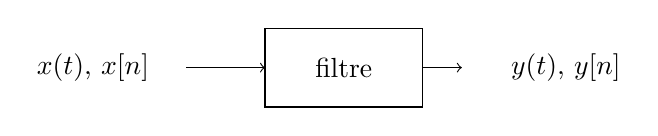
\begin{tikzpicture}

	\draw (2.15,0) node[left] {$x(t)$, $x[n]$};

	
	\draw[->] (2.5,0)-- (3.5,0);
	\draw (3.5,-0.5) rectangle(5.5,0.5) ;
	\draw (4.5,0) node {filtre};

	\draw[->] (5.5,0)-- (6,0);

	\draw (6.5,0) node[right] {$y(t)$, $y[n]$};

	\end{tikzpicture}
\end{center}
}

\only<3->{
\vspace{1 cm}
\begin{block}{}
"En traitement du signal, un filtre est un dispositif ou un processus permettant de retirer des composantes ou des parties indésirables d'un signal." (wikipedia.org)
\end{block}
}
\end{frame}

\subsection{Caractérisation de filtres}
\begin{frame}
\frametitle{Comment caractérise-t-on un filtre ?}
\textbf{Quels termes utiliseriez-vous pour définir un filtre ?}
\vspace{1cm}
\begin{itemize}
\item<2-> Analogique/Numérique
\item<3-> Actif/Passif (analogique)
\item<4-> Causal/Non causal (numérique)
\item<5-> Linéaire/Non linéaire 
\item<6-> Invariant/Non invariant dans le temps
\end{itemize}
\only<7->
{
\begin{block}{}
Objet du cours: Filtres numériques, causaux, linéaires, invariants dans le temps.
\end{block}
}
\end{frame}



\subsection{Linéarité}
\begin{frame}
\frametitle{Notion de linéarité}
\textbf{Question: Que veut dire linéaire en ingénierie des systèmes/automatique/traitement du signal ? \label{linéaire ?} }\\
\vspace{1 cm}
\only<2->
{
Soit $f : x \in \mathbb{R} \rightarrow f(x) \in \mathbb{R} $ et $(x_1,x_2,a,b) \in \mathbb{R}^4$
\\}
\vspace{1 cm}
\only<3->
{
$f$ linéaire si\\
\vspace{0.5 cm}
\begin{block}{}
\[f(a x_1 + b x_2) = a f(x_1) + b f(x_2)\]
\end{block}
}

\end{frame}

\begin{frame}
\frametitle{Notion de linéarité}
 \textbf{Linéarité : application}
\textbf{Soit $x$ une variable réelle, les fonctions suivantes sont-elles linéaires ?}:
 \vspace{0.5cm}
\begin{itemize}
\item<2-> $f(x) = a x^2 + b x + c$ (avec $a$, $b$ et $c$ des constantes réelles positives)
\item<3-> $f(x) = \sqrt{x^2}$
\item<4-> $f(x) = a$ (constante réelle positive)
\item<5-> $f(x) = \ln(x)$
\item<6-> $f(x) = \frac{1}{a x + b}$
\end{itemize}
\vspace{1cm}
\only<8->
{
Aucune de ces fonctions n'est linéaire...
}
\end{frame}

\begin{frame}
\frametitle{Notion de linéarité: capteurs}
\textbf{Que vous évoque la notion de linéarité dans le cadre des capteurs ?}\\
\vspace{1 cm}
\only<2->{
\usetikzlibrary {decorations.pathmorphing} 
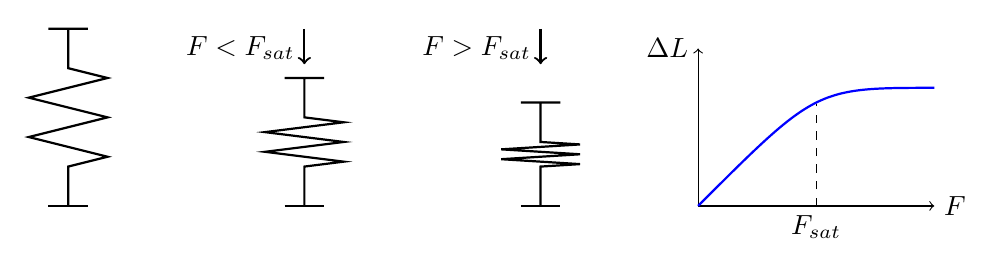
\begin{tikzpicture}

	%spring 
	\draw[thick] (-0.25,0)--(0.25,0);
	\draw[thick] (0,0)--(0,0.5)--++(0.5,0.125) --++(-1,0.25) --++(1,0.25) --++(-1,0.25) --++(1,0.25) --++(-0.5,0.125)--++(0,0.5)--++(-0.25,0)--++(0.5,0); 
		
%			\begin{scope}[xshift = 1.5cm]
%				\draw[thick,<->] (0,2.25)--(0,1.75); 
%				\draw (0,2) node[left] {$\Delta L$};
%			\end{scope}		
		
		
			\begin{scope}[xshift = 3cm]
			\draw[thick] (-0.25,0)--(0.25,0);
			\draw[thick] (0,0)--(0,0.5)--++(0.5,0.125/2) --++(-1,0.25/2) --++(1,0.25/2) --++(-1,0.25/2) --++(1,0.25/2) --++(-0.5,0.125/2)--++(0,0.5)--++(-0.25,0)--++(0.5,0); 
	\end{scope}
	
			\begin{scope}[xshift = 3cm]
				\draw[thick,->] (0,2.25)--(0,1.80); 
				\draw (0,2) node[left] {$F<F_{sat}$};
			\end{scope}	
	
	
	\begin{scope}[xshift = 6cm]
	\draw[thick] (-0.25,0)--(0.25,0);
			\draw[thick] (0,0)--(0,0.5)--++(0.5,0.125/4) --++(-1,0.25/4) --++(1,0.25/4) --++(-1,0.25/4) --++(1,0.25/4) --++(-0.5,0.125/4)--++(0,0.5)--++(-0.25,0)--++(0.5,0); 
	\end{scope}
	
		\begin{scope}[xshift = 6cm]
				\draw[thick,->] (0,2.25)--(0,1.80); 
				\draw (0,2) node[left] {$F>F_{sat}$};
			\end{scope}	
	

	
	\begin{scope}[xshift= 8cm] 
	\draw[->] (0,0)--(3,0) node[right] {$F$};
	\draw[->] (0,0)--(0,2) node[left] {$\Delta L$};	
	\draw[thick,blue] (0,0) .. controls (1.5,1.5) .. (3,1.5);
	\draw[dashed,black] (1.5,0)node[below]{$F_{sat}$} --(1.5,1.3) ;
	\end{scope}
\end{tikzpicture}
}
\only<3->{
\begin{block}{}
Le capteur sort de sa zone de linéarité lorsqu'on perd la relation linéaire/affine entre l'entrée et la sortie
\end{block}
}
\end{frame} 



\subsection{Invariance dans le temps}
\begin{frame}
\frametitle{Notion d'invariance dans le temps}
Prérequis : Notion de retard d'une fonction \\
\only<2->{
\vspace{1 cm} 
Soit $x : t \in \mathbb{R} \rightarrow x(t) \in \mathbb{R} $ \\

\vspace{1 cm} 
La fonction $x(t)$ retardé de $\tau \in \mathbb{R}$ s'écrit $x(t-\tau)$\\
\vspace{1 cm}
}

\only<3->{
La suite $x[n]$ retardé de $k \in \mathbb{N}$ s'écrit $x[n-k]$
}

\end{frame}

\begin{frame}
\frametitle{Invariance dans le temps}

\begin{block}{Attention}
La notion d'invariance dans le temps est ici appliqué au \textbf{filtre/système} faisant la correspondance entre les \textbf{fonctions} d'entrée et de sortie 
\end{block}
\end{frame}


\begin{frame}
\frametitle{Invariance dans le temps}
Soit $F$ un filtre de telle sorte que, pour $x(t)$ et $y(t)$ deux fonctions , $ \forall \; t \in \mathbb{R}, \; y(t) = F(x(t))$ ou $ \forall \; n \in \mathbb{N}, \; y[n] = F(x[n])$ \\

\only<2->
{
\vspace{1cm} 
le filtre $F$  est dit \textbf{invariant dans le temps} si \\
\vspace{1cm}
\begin{center}
$\forall \tau \in \mathbb{R}, \;\; F(x(t-\tau)) = y(t-\tau)$\\
\vspace{0.7 cm}
$\forall k \in \mathbb{N}, \;\; F(x[n-k]) = y[n-k]$\\
\end{center}
}

\only<3->
{ 
\begin{block}{}
	En résumé, la réponse d'un filtre/système invariant dans le temps ne doit pas dépendre du moment où on l'utilise
\end{block} 
}

\end{frame}


\subsection{Système linéaire et invariant dans le  temps (LIT)}

\begin{frame}
\frametitle{Système linéaire et invariant dans le  temps (LIT) }

Un système F est linéaire invariant dans le temps si :
\begin{itemize}
\item La sortie correspondant à une combinaison linéaire de signaux d'entrée est la combinaison linéaire des signaux de sortie correspondant aux entrées prises séparément\\
\item la réponse d'un filtre/système invariant dans le temps ne doit pas dépendre du moment où on l'utilise\\
\end{itemize}

\end{frame} 

\begin{frame} 
\frametitle{Système linéaire et invariant dans le temps (LIT) }
Soit un signal d'entrée $x$ (continue ou discret) et $F$ un filtre/système LIT\\
\vspace{1 cm}
\begin{columns}
\column{70mm}
\begin{center}
$x(t) = \displaystyle \int x(\tau) \delta(t-\tau) d\tau$\\
\only<2->{
\vspace{0.5cm}
$F(x(t)) = y(t)$\\
$ = F( \displaystyle \int x(\tau) \delta(t-\tau) d\tau)$\\
\vspace{0.5cm}
}

\only<3->{
F linéaire donc, \\
\vspace{0.5cm}
$F(x(t)) = y(t) $\\
$= \displaystyle \int F (x(\tau) \delta(t-\tau) d\tau)$
}
\end{center}

\column{60mm}
\begin{center}
$x[n] =  \displaystyle \sum x[k] \delta[n-k] $ \\
\vspace{0.5cm}

\only<2->{
$F(x[n]) = y[n] $\\
$= F(\displaystyle \sum x[k] \delta[n-k]) $ \\
\vspace{0.5cm}
}

\only<3->{
F linéaire donc, \\
\vspace{0.5cm}
$F(x[n]) = y[n] $\\
$ = \displaystyle \sum F( x[k] \delta[n-k]) $ \\
}

\end{center}
\end{columns}
\end{frame}

\begin{frame} 
\frametitle{Système linéaire et invariant dans le temps (LIT) }
Soit un signal d'entrée $x$ (continue ou discret) et $F$ un filtre/système LIT\\
\vspace{1 cm}
\begin{columns}
\column{70mm}
\begin{center}
$F(x(t)) = y(t) $\\
$= \displaystyle \int F (x(\tau) \delta(t-\tau) d\tau)$\\
\vspace{0.5cm}

$F$ s'applique aux fonctions de $t$\\
\vspace{0.5cm}

$y(t) = \displaystyle \int x(\tau) F(\delta(t-\tau) )d\tau$\\
\vspace{0.5cm}

\end{center}

\column{60mm}
\begin{center}
$F(x[n]) = y[n] $\\
$ = \displaystyle \sum F( x[k] \delta[n-k]) $ \\
\vspace{0.5cm}

$F$ s'applique aux suites sur $n$\\
\vspace{0.5cm}

$ y[n] = \displaystyle \sum x[k]  F(\delta[n-k]) $ \\
\vspace{0.5cm}


\end{center}
\end{columns}
\end{frame}

\begin{frame} 
\frametitle{Système linéaire et invariant dans le temps (LIT) }
Soit un signal d'entrée $x$ (continue ou discret) et $F$ un filtre/système LIT\\
\vspace{1 cm}
\begin{columns}
\column{70mm}
\begin{center}
$y(t) = \displaystyle \int x(\tau) F(\delta(t-\tau) )d\tau$\\
\vspace{0.5cm}

Puisque $F$ invariant dans le temps,\\
\vspace{0.5cm}

$y(t) = \displaystyle \int x(\tau) h(t-\tau) d\tau$\\
\vspace{0.5cm}

avec $h[t]$ la\\ \textbf{réponse impulsionnelle} du filtre $F$

\end{center}

\column{60mm}
\begin{center}

$ y[n] = \displaystyle\sum x[k]  F(\delta[n-k]) $ \\
\vspace{0.5cm}

Puisque $F$ invariant dans le temps,\\
\vspace{0.5cm}

$ y[n] = \displaystyle\sum x[k]  h[n-k] $ \\
\vspace{0.5cm}

avec $h[n]$ la\\ \textbf{réponse impulsionnelle} du filtre $F$

\end{center}
\end{columns}
\begin{block}{}
Ces deux relations sont ce qu'on appelle \textbf{l'équation de convolution}
\end{block}
\end{frame}

\begin{frame}
\frametitle{Système linéaire et invariant dans le temps (LIT)}
Le fait que le sytème soit LIT et les équations de convolutions sous-tendent: \\
\vspace{1cm}
\begin{itemize}
\item La possibilité d'écrire une \textbf{fonction de transfert}
\item La possibilité de \textbf{prédire/calculer le comportement} d'un système "arbitraire"
\item La possibilité de créer des \textbf{systèmes complexes} au comportement connu à partir de \textbf{cellules "simples"}
\end{itemize}

\end{frame} 

\begin{frame} 
\frametitle{Structure du cours}
\begin{enumerate}
\item Outils mathématiques généraux  
\item Signaux numériques : Spécificités 
\item Filtres numériques : Généralités 
\item Filtres à réponse impulsionnelle finie/Filtres non-récursifs 
\item Filtres à réponse impulsionnelle infinie/Filtres récursifs 
\end{enumerate}
\end{frame} 

\section{Outils Mathématiques}
\subsection{Transformée de Laplace}

\begin{frame}
\frametitle{Transformée de Laplace}
\textbf{Que vous évoque la transformée de Laplace ?}\\

\vspace{1cm}

\only<2->
{
	Transformée de Laplace monolatérale : $L\{f\}(s) = \displaystyle \int^{\infty}_{0} f(t) e^{-st} \; dt$\\ 
	\vspace{0.3cm}
	Transformée de Laplace bilatérale : $L\{f\}(s) = \displaystyle \int^{\infty}_{-\infty} f(t) e^{-st} \; dt$
}

\only<3->
{
\begin{block}{}
Utile, entre autre, pour analyser des systèmes dynamiques de façon rapide.
\end{block}
}

\end{frame}

\begin{frame}
\frametitle{Propriétés de la transformée de Laplace}
\begin{itemize}
\item<2-> Linéarité: \only<3->{ $L\{af+g\}(s) = a L\{ f\}(s) + L \{ g \} (s)$}
\item<4-> Dérivation : \only<5->{$ L\{f'\}(s) = \; s L\{f \}(s)$}
\item<5-> Intégration : \only<6->{$ L\{F\}(s) = \frac{\displaystyle 1}{\displaystyle s} L\{f \}(s) $}
\item<7-> Convolution : \only<8->{$ L\{f \star g \} = L\{f \}(s) \cdot L \{ g \} (s)  $}
\end{itemize}

\end{frame}

\begin{frame} 
\frametitle{Transformée de Laplace}

\textbf{Exercice: Calculer les transformées de Laplace suivantes}\\
\vspace{1cm}
\begin{itemize}
\item $u(t)$ (échelon de heaviside)
\item $r(t) = t$ (rampe)
\item $f(t) = e^{-at}$ (exponentielle décroissante)
\item $\delta (t)$ (impulsion de dirac) 
\item $sin(\omega t)$
\end{itemize}

\end{frame} 

\begin{frame} 
\frametitle{Transformée de Laplace}

\textbf{Exercice: Calculer les transformées de Laplace suivantes}\\
\vspace{1cm}
\begin{itemize}
\item $u(t)$  \only<2->{$\rightarrow \frac{\displaystyle 1}{\displaystyle p} $} 
\item $r(t) = t$  \only<3->{$\rightarrow \frac{\displaystyle 1}{ \displaystyle p^2} $} 
\item $f(t) = e^{-at}$  \only<4->{$\rightarrow \frac{\displaystyle 1}{\displaystyle p+a} $}
\item $\delta (t)$ \only<5->{$\rightarrow 1$} 
\item $sin(\omega t)$ = \only<6->{$\rightarrow \frac{\displaystyle \omega_0^2}{ \displaystyle p^2 + \omega_0^2} $}
\end{itemize}

\end{frame}

\subsection{Transformée de Fourier et lien avec la transformée de Laplace}

\subsubsection{Transformée de Fourier}


\begin{frame}
\frametitle{Transformée de Fourier}
\textbf{Question: Quelle est pour vous le lien entre transformée de Laplace et transformée de Fourier}\\
\vspace{1 cm}
\only<2->
{
\begin{center}
	$L\{f\}(s) = \displaystyle \int^{\infty}_{-\infty} f(t) e^{-st} \; dt $ \only<3->{$ \rightarrow TF\{ f \}(\nu) = \displaystyle \int^{\infty}_{-\infty} f(t) e^{-j2\pi \nu t} dt $}
\end{center} 
}

\only<4->{
\begin{block}{}
La transformée de Fourier peut s'écrire commes un cas particulier de la transformée de Laplace bilatérale.
\end{block}
}
\end{frame}

\subsubsection{Spectre}
\begin{frame}
\frametitle{Transformée de Fourier}
\[ TF\{ f \}(\nu) = \displaystyle \int^{\infty}_{-\infty} f(t) e^{-j2\pi \nu t} dt   = F(\nu) \]\\
\vspace{1cm}

La fonction $F(\nu)$ est généralement désigné comme \textbf{spectre fréquentiel} de $f(t)$ \\

\vspace{1cm}
\only<2->{
$F(\nu)$ est une fonction \textbf{complexe} 
}

\only<3->{
\begin{block}{}
Comment le représenter ? 
\end{block}
}
\end{frame}

\begin{frame}
\frametitle{Transformée de Fourier : Spectre }

Comment représenter $F(\nu)$  ? \\

\vspace{1cm} 

2 possibilités pour représenter un nombre complexe $z$: 

\begin{itemize}
\item $z = a+ ib$
\item $z = r\cdot e^{i \theta}$
\end{itemize} 

\vspace{1 cm}

\only<2->{
\begin{block}{}
Dans la grande majorité des cas c'est la représentation module/argument $z = r\cdot e^{i \theta}$ qui est utilisée.
\end{block}
}

\subsubsection{Module et phase: exemples}

\vspace{1cm}
\only<3->
{
On va prendre la fonction $g_1(t) = \cos(2 t)$ pour illustrer
}

\end{frame} 

\begin{frame}
\frametitle{Transformée  de Fourier : Spectre}
Spectre de $g_1(t) = \cos(2 t)$ \\

\only<2->{
\begin{center}
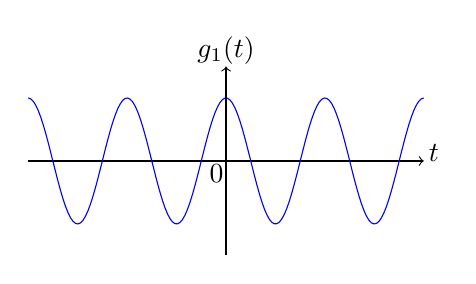
\begin{tikzpicture}
\begin{scope}[scale=0.4]
	\draw[->] (-6.28,0)-- (6.28,0);
\draw (-0.3,-0.4) node {0};
\draw[->] (0,-3)-- (0,3);
\draw (2.1*pi,0.25) node {$t$};
\draw (0,3.5) node {$g_1(t)$};

\draw[domain=-6.28:6.28,color=blue,samples=160] plot (\x,{2*cos(2*\x r)});	
\end{scope}
\end{tikzpicture}
\end{center}
}

\only<3->{
Soit $z = a +ib$, alors $|z|=$\only<2->{$r = \sqrt{a^2 + b^2}$}
et $arg(z) = \theta = \arctan(\frac{\displaystyle b}{\displaystyle a})$
}

\vspace{0.4 cm} 

\only<4->{
 $$TF\{ g_1 \}(\nu) = \int^{\infty}_{-\infty} g_1(t) e^{-2\pi j \nu t} \; dt$$ \only<5->{$$= \frac{\displaystyle \delta(\nu - 1/\pi) + \delta(\nu + 1/\pi)}{\displaystyle 2}
$$}}

\end{frame}

\begin{frame}
\frametitle{Transformée  de Fourier : Spectre}
 $$TF\{ g_1 \}(\nu) = \int^{\infty}_{-\infty} g_1(t) e^{-2\pi j \nu t} \; dt= \frac{\displaystyle \delta(\nu - 1/\pi) + \delta(\nu + 1/\pi)}{\displaystyle 2}$$\\
 
 \vspace{1cm}
 \only<2->{
 $$|TF\{ g_1 \}(\nu)| = |G_1(\nu)| = \frac{\displaystyle \delta(\nu - 1/\pi) + \delta(\nu + 1/\pi)}{\displaystyle 2} $$
 }
 
\only<3->{
\begin{center}
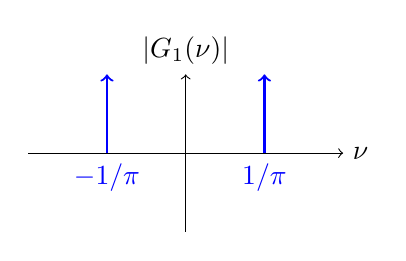
\begin{tikzpicture}
\draw[->] (-2,0)--(2,0) node[right]{$\nu$};
\draw[->] (0,-1)--(0,1) node[above]{$|G_1(\nu)|$};
\draw[->,blue,thick] (-1,0) node[below]{$-1/\pi$}--(-1,1) ;
\draw[->,blue,thick] (1,0) node[below]{$1/\pi$}--(1,1) ;
\end{tikzpicture}
\end{center}
}
\end{frame}

\begin{frame}
\frametitle{Transformée de Fourier : Spectre}
$$G_1(\nu) = \frac{\displaystyle \delta(\nu - 1/\pi) + \delta(\nu + 1/\pi)}{\displaystyle 2} $$\\

\vspace{0.6cm}
\only<2->{
$$arg(G_1(\nu)) = $$ \only<3->{ $$\arctan(\frac{0}{\frac{\displaystyle \delta(\nu - 1/\pi) + \delta(\nu + 1/\pi)}{\displaystyle 2}}) = 0$$}\\
}
\vspace{0.6cm}
\only<3->{
\begin{center}
\begin{tikzpicture}
\draw[->] (-2,0)--(2,0) node[right]{$\nu$};
\draw[->] (0,-1)--(0,1) node[above]{$arg(G_1(\nu))$};
\draw[->,blue,thick] (-1,0) node[below]{$-1/\pi$}--(-1,0) ;
\draw[->,blue,thick] (1,0) node[below]{$1/\pi$}--(1,0) ;
\end{tikzpicture}
\end{center}
}

\end{frame}

\begin{frame}
\frametitle{Transformée  de Fourier : Spectre}
En résumé, \\
\vspace{0.3cm}
\[g_1(t) = \cos(2 t) \rightarrow  G_1(\nu) = \frac{\displaystyle \delta(\nu - 1/\pi) + \delta(\nu + 1/\pi)}{\displaystyle 2} \]

\begin{columns}
\column{60mm}
\only<2->{
\[|G_1(\nu)| = \frac{\displaystyle \delta(\nu - 1/\pi) + \delta(\nu + 1/\pi)}{\displaystyle 2}\]\\
}
\vspace{0.1cm}
\only<3->
{
\begin{center}
\begin{tikzpicture}
\draw[->] (-2,0)--(2,0) node[right]{$\nu$};
\draw[->] (0,-1)--(0,1) node[above]{$|G_1(\nu)|$};
\draw[->,blue,thick] (-1,0) node[below]{\scriptsize $-1/\pi$}--(-1,1) ;
\draw[->,blue,thick] (1,0) node[below]{\scriptsize $1/\pi$}--(1,1) ;
\end{tikzpicture}
\end{center}
}

\column{60mm}
\only<2->{
$$arg(G_1(\nu))  = 0 $$ \\
}
\vspace{0.65cm}
\only<3->
{
\begin{center}
\begin{tikzpicture}
\draw[->] (-2,0)--(2,0) node[right]{$\nu$};
\draw[->] (0,-1)--(0,1) node[above]{$arg(G_1(\nu))$};
\draw[->,blue,thick] (-1,0) node[below]{\scriptsize $-1/\pi$}--(-1,0) ;
\draw[->,blue,thick] (1,0) node[below]{ \scriptsize $1/\pi$}--(1,0) ;
\end{tikzpicture}
\end{center}
}
\end{columns}
\end{frame}

\begin{frame}
\frametitle{Transformée  de Fourier : Spectre}
Spectre de $g_2(t) = 0.55\cos(2 t) + 0.45 \cos(4 t + \frac{\pi}{3})$ \\
\only<2->{
\begin{center}
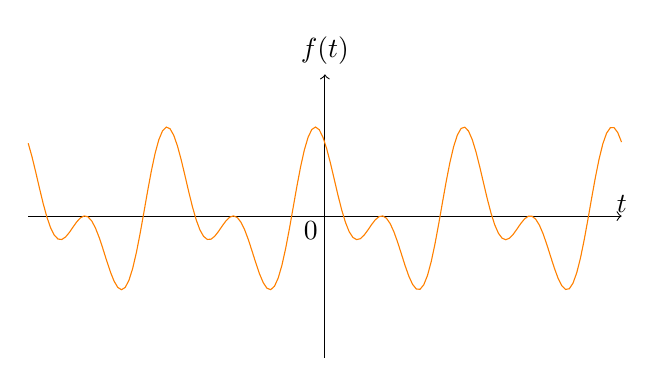
\begin{tikzpicture}
\begin{scope}[scale=0.6]
	\draw[->] (-6.28,0)-- (6.28,0);
\draw (-0.3,-0.3) node {0};
\draw[->] (0,-3)-- (0,3);
\draw (2*pi,0.25) node {$t$};
\draw (0,3.5) node {$f(t)$};
%\draw (4.5,-0.3) node {1};

		\draw[domain=-6.28:6.28,color=orange,samples=160] plot (\x,{2*(0.55*cos(2*\x r)+ 0.45*cos(2*2*(\x+3.14/12) r))});
	\end{scope}
	\end{tikzpicture}
\end{center}
}
\end{frame}

\begin{frame}
\frametitle{Transformée  de Fourier : Spectre}

\[ TF\{ g_2 \}(f) = G_2(\nu)\]\\
\[ =   \frac{0.55}{2}(\delta(\nu+1/\pi) + \delta(\nu-1/\pi)) + \frac{0.45}{2}(\delta(\nu+2/\pi) + \delta(\nu-2/\pi)) \cdot e^{2 j \pi \frac{\pi}{3} \nu }\]\\

\vspace{0.5 cm}

\[|G_2(\nu)| = \bigl[(\frac{0.55}{2}(\delta(\nu+1/\pi) + \delta(\nu-1/\pi))+ \] \\
\[ \frac{0.45}{2}(\delta(\nu+2/\pi) + \delta(\nu-2/\pi)) \cdot  \cos(2\frac{\pi^2}{3} \nu))^2 \]\\
\[+(\frac{0.45}{2}(\delta(\nu+2/\pi) + \delta(\nu-2/\pi)) \cdot  \sin(2\frac{\pi^2}{3} \nu))^2 \bigr] ^{1/2} \]

\end{frame}

\begin{frame} 
\frametitle{Transformée  de Fourier : Spectre}

\[|G_2(\nu)| = \bigl[(\frac{0.55}{2}(\delta(\nu+1/\pi) + \delta(\nu-1/\pi))+ \] \\
\[ \frac{0.45}{2}(\delta(\nu+2/\pi) + \delta(\nu-2/\pi)) \cdot  \cos(2\frac{\pi^2}{3} \nu))^2 \]\\
\[+(\frac{0.45}{2}(\delta(\nu+2/\pi) + \delta(\nu-2/\pi)) \cdot  \sin(2\frac{\pi^2}{3} \nu))^2 \bigr] ^{1/2} \]\\

\vspace{0.5cm}
\only<2->{
\begin{center}
\begin{tikzpicture}
\draw[->] (-2.5,0)--(2.5,0) node[right]{$\nu$};
\draw[->] (0,-1)--(0,1) node[above]{$|G_2(\nu)|$};
\draw[->,orange,thick] (-1,0) node[below]{\scriptsize $-1/\pi$}--(-1,0.55) ;
\draw[->,orange,thick] (1,0) node[below]{\scriptsize $1/\pi$}--(1,0.55) ;
\draw[->,orange,thick] (-2,0) node[below]{\scriptsize $-2/\pi$}--(-2,0.225) ;
\draw[->,orange,thick] (2,0) node[below]{\scriptsize $2/\pi$}--(2,0.225) ;
\end{tikzpicture}
\end{center}
}
\end{frame}

\begin{frame}
\frametitle{Transformée  de Fourier : Spectre}
\[ arg(G_2(\nu)) = \]\\
\[ \arctan\bigl( \frac{\frac{0.45}{2}(\delta_2) \cdot  \sin(2\frac{\pi^2}{3} \nu)}{\frac{0.55}{2}(\delta_1)+
 \frac{0.45}{2}(\delta_2) \cdot  \cos(2\frac{\pi^2}{3} \nu)}\bigr) \]\\
 \vspace{0.3cm} 
 \only<2->{
 \[arg(G_2(\nu)) = 2\frac{\pi^2}{3} \nu \]\\
 }

 \vspace{0.3cm}
 \only<3->
{
\begin{center}
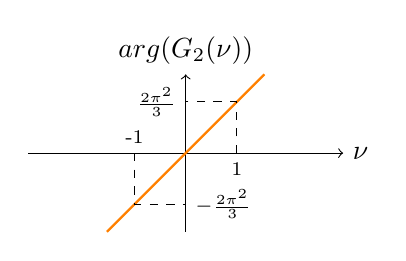
\begin{tikzpicture}
\draw[->] (-2,0)--(2,0) node[right]{$\nu$};
\draw[->] (0,-1)--(0,1) node[above]{$arg(G_2(\nu))$};
\draw[orange,thick] (-1,-1) --(1,1) ;
\draw[dashed] (-0.65,0)node[above]{\scriptsize -1} --(-0.65,-0.65)--(0,-0.65)node[right]{\scriptsize $-\frac{2\pi^2}{3}$} ;
\draw[dashed] (0.65,0)node[below]{\scriptsize 1} --(0.65,0.65)--(0,0.65)node[left]{\scriptsize $\frac{2\pi^2}{3}$} ;
\end{tikzpicture}
\end{center}
}
\end{frame}

\begin{frame}
\frametitle{Transformée  de Fourier : Spectre}
\[ TF\{ g_2 \}(f) = G_2(\nu)\]\\
\[ =   \frac{0.55}{2}(\delta(\nu+1/\pi) + \delta(\nu-1/\pi)) + \frac{0.45}{2}(\delta(\nu+2/\pi) + \delta(\nu-2/\pi)) \cdot e^{2 j \pi \frac{\pi}{3} \nu }\]\\

\vspace{0.3cm}
\begin{columns}
\column{60mm}
\only<2->{
\begin{center}
\begin{tikzpicture}
\draw[->] (-2.5,0)--(2.5,0) node[right]{$\nu$};
\draw[->] (0,-1)--(0,1) node[above]{$|G_2(\nu)|$};
\draw[->,orange,thick] (-1,0) node[below]{\scriptsize $-1/\pi$}--(-1,0.55) ;
\draw[->,orange,thick] (1,0) node[below]{\scriptsize $1/\pi$}--(1,0.55) ;
\draw[->,orange,thick] (-2,0) node[below]{\scriptsize $-2/\pi$}--(-2,0.225) ;
\draw[->,orange,thick] (2,0) node[below]{\scriptsize $2/\pi$}--(2,0.225) ;
\end{tikzpicture}
\end{center}

}
\column{60mm}
\only<2->{
\begin{center}
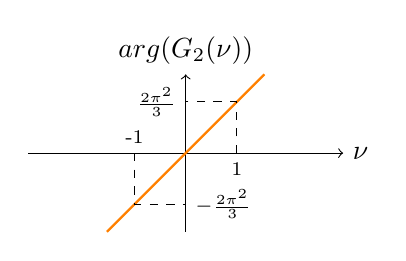
\begin{tikzpicture}
\draw[->] (-2,0)--(2,0) node[right]{$\nu$};
\draw[->] (0,-1)--(0,1) node[above]{$arg(G_2(\nu))$};
\draw[orange,thick] (-1,-1) --(1,1) ;
\draw[dashed] (-0.65,0)node[above]{\scriptsize -1} --(-0.65,-0.65)--(0,-0.65)node[right]{\scriptsize $-\frac{2\pi^2}{3}$} ;
\draw[dashed] (0.65,0)node[below]{\scriptsize 1} --(0.65,0.65)--(0,0.65)node[left]{\scriptsize $\frac{2\pi^2}{3}$} ;
\end{tikzpicture}
\end{center}

}

\end{columns}

\end{frame}

\begin{frame}
\frametitle{Transformée  de Fourier : Spectre}
La phase a son importance... \\
\vspace{0.3cm}
Si on prend  $g_3(t) = 0.55\cos(2 t) + 0.45 \cos(4 t)$...\\
\vspace{0.3cm}
\begin{columns}
\column{60mm}
\only<2->{



\begin{center}
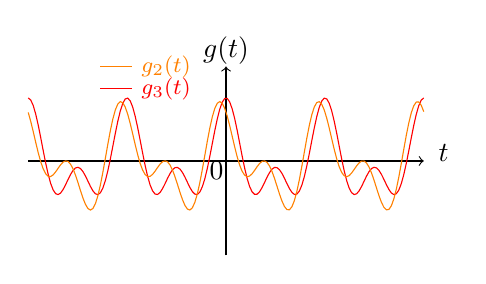
\begin{tikzpicture}
	\begin{scope}[scale=0.4]
	\draw[->] (-6.28,0)-- (6.28,0);
\draw (-0.3,-0.3) node {0};
\draw[->] (0,-3)-- (0,3);
\draw (2.2*pi,0.25) node {$t$};
\draw (0,3.5) node {$g(t)$};

	\draw[domain=-6.28:6.28,color=red,samples=160] plot (\x,{2*(0.55*cos(2*\x r)+ 0.45*cos(2*2*\x r))});
	
		\draw[domain=-6.28:6.28,color=orange,samples=160] plot (\x,{2*(0.55*cos(2*\x r)+ 0.45*cos(2*2*(\x+3.14/12) r))});
		
		\draw[orange] (-4,3)--(-3,3)node[right] {\footnotesize $g_2(t)$};
		\draw[red] (-4,2.3)--(-3,2.3)node[right] {\footnotesize $g_3(t)$};
	\end{scope}
	\end{tikzpicture}
\end{center}


\only<4->
{
L'ajout d'un déphasage à une des composantes change la forme du signal et la phase (qui devient nulle) mais PAS le module
}

\column{60mm}
\only<3->{
\begin{center}
\begin{tikzpicture}
\draw[->] (-2.5,0)--(2.5,0) node[right]{$\nu$};
\draw[->] (0,-1)--(0,1) node[above]{$|G_3(\nu)|$};
\draw[->,red,thick] (-1,0) node[below]{\scriptsize $-1/\pi$}--(-1,0.55) ;
\draw[->,red,thick] (1,0) node[below]{\scriptsize $1/\pi$}--(1,0.55) ;
\draw[->,red,thick] (-2,0) node[below]{\scriptsize $-2/\pi$}--(-2,0.225) ;
\draw[->,red,thick] (2,0) node[below]{\scriptsize $2/\pi$}--(2,0.225) ;
\end{tikzpicture}
\end{center}
\vspace{0cm}
\begin{center}
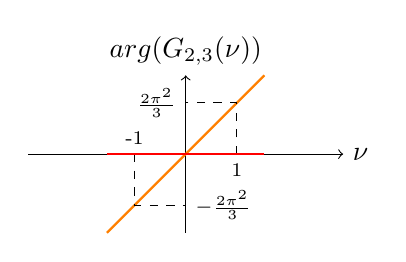
\begin{tikzpicture}
\draw[->] (-2,0)--(2,0) node[right]{$\nu$};
\draw[->] (0,-1)--(0,1) node[above]{$arg(G_{2,3}(\nu))$};
\draw[orange,thick] (-1,-1) --(1,1) ;
\draw[dashed] (-0.65,0)node[above]{\scriptsize -1} --(-0.65,-0.65)--(0,-0.65)node[right]{\scriptsize $-\frac{2\pi^2}{3}$} ;
\draw[dashed] (0.65,0)node[below]{\scriptsize 1} --(0.65,0.65)--(0,0.65)node[left]{\scriptsize $\frac{2\pi^2}{3}$} ;
\draw[red,thick] (-1,0) --(1,0) ;
\end{tikzpicture}
\end{center}
}
} 
\end{columns}
\vspace{0.3cm}

\end{frame}

\subsection{Concepts utile dans le domaine de Fourier}

\begin{frame}
\frametitle{Choses à savoir sur la Transformée de Fourier}
Il y a des petites "lois" qu'il peut être utile d'avoir à l'esprit lorsqu'on manipule des fonctions et leurs spectres...\\

\vspace{0.1cm}
\only<2->
{
1a.\textbf{ Extension temporelle faible = Extension fréquentielle forte}
}

\only<3->{
\begin{center}
\begin{tikzpicture}
\draw[->] (-2,0)--(2,0) node[right]{$t$};
\draw[->] (0,-1)--(0,1) node[above]{$f(t)$};
\draw[thick,blue] (-2,0)--(0,0)--(0,1)--(0,0)--(2,0);

\begin{scope}[xshift=6cm]
\draw[->] (-2,0)--(2,0) node[right]{$\nu$};
\draw[->] (0,-1)--(0,1) node[above]{$F(\nu)$};
\draw[thick,blue] (-2,0.5)--(2,0.5);
\end{scope}
\end{tikzpicture}
\end{center}
}

\only<4->
{
1b.\textbf{ Extension temporelle forte = Extension fréquentielle faible}
}

\only<4->{
\begin{center}
\begin{tikzpicture}
\draw[->] (-2,0)--(2,0) node[right]{$t$};
\draw[->] (0,-1)--(0,1) node[above]{$f(t)$};
\draw[thick,blue] (-2,0.5)--(2,0.5);

\begin{scope}[xshift=6cm]
\draw[->] (-2,0)--(2,0) node[right]{$\nu$};
\draw[->] (0,-1)--(0,1) node[above]{$F(\nu)$};
\draw[thick,blue] (-2,0)--(0,0)--(0,1)--(0,0)--(2,0);
\end{scope}
\end{tikzpicture}
\end{center}
}

\end{frame} 

\begin{frame}
\frametitle{Choses à savoir sur la Transformée de Fourier}
2. Périodicité temporelle et spectre 


\only<2->{
\begin{tikzpicture}
\draw[->] (2.5,0) node[below] {0} -- (2.5,1.5)node[above] {$e(t)$};
\draw[->] (0,0)-- (5,0) node[right] {$t$};

\draw[thick,blue] (2,0)--(2.25,0)--(2.25,1)--(2.75,1)--(2.75,0)--(3,0);

\begin{scope}[xshift=1cm]
\draw[thick,blue] (2,0)--(2.25,0)--(2.25,1)--(2.75,1)--(2.75,0)--(3,0);
\draw[dashed,black] (2.5,0) node[below]{$T$}--(2.5,1);
\end{scope}

\begin{scope}[xshift=2cm]
\draw[thick,blue] (2,0)--(2.25,0)--(2.25,1)--(2.75,1)--(2.75,0)--(3,0);
\end{scope}


\begin{scope}[xshift=-1cm]
\draw[thick,blue] (2,0)--(2.25,0)--(2.25,1)--(2.75,1)--(2.75,0)--(3,0);
\end{scope}

\begin{scope}[xshift=-2cm]
\draw[thick,blue] (2,0)--(2.25,0)--(2.25,1)--(2.75,1)--(2.75,0)--(3,0);
\end{scope}



\begin{scope}[xshift=7cm]
\draw[->] (2.5,0) node[below] {0} -- (2.5,1.5)node[above] {$E(\nu)$};
\draw[->] (0,0)-- (5,0) node[right] {$\nu$};
\draw[ domain=0.1:4.9,color=blue,samples=24] plot[ycomb] (\x,{80*abs(sin(5*3.14*\x r -5*3.14*2.5r )/(5*3.14*\x r-5*3.14*2.5 r))});
\draw[<->] (3.25,-0.3)--(3.45,-0.3) node[below left] {$\frac{1}{T}$};
\end{scope}
\end{tikzpicture}
}

\only<3->{
\begin{tikzpicture}
\draw[->] (2.5,0) node[below] {0} -- (2.5,1.5)node[above] {$e(t)$};
\draw[->] (0,0)-- (5,0) node[below right] {$t$};

\draw[thick,blue] (1,0)--(2.25,0)--(2.25,1)--(2.75,1)--(2.75,0)--(4,0);


\begin{scope}[xshift=2cm]
\draw[thick,blue] (1,0)--(2.25,0)--(2.25,1)--(2.75,1)--(2.75,0)--(3,0);
\end{scope}


\begin{scope}[xshift=-2cm]
\draw[thick,blue] (2,0)--(2.25,0)--(2.25,1)--(2.75,1)--(2.75,0)--(4,0);
\end{scope}



\begin{scope}[xshift=7cm]
\draw[->] (2.5,0) node[below] {0} -- (2.5,1.5)node[above] {$E(\nu)$};
\draw[->] (0,0)-- (5,0) node[right] {$\nu$};
\draw[ domain=0.1:4.9,color=blue,samples=96] plot[ycomb] (\x,{80*abs(sin(5*3.14*\x r -5*3.14*2.5r )/(5*3.14*\x r-5*3.14*2.5 r))});
%\draw[<->] (3.25,-0.3)--(3.45,-0.3) node[below left] {$\frac{1}{T}$};
\end{scope}
\end{tikzpicture}
}

\only<4->{
Pertinent lorsqu'il est question d'échantillonnage...
}
\end{frame}


\subsection{Signaux Numériques}
\begin{frame}
\frametitle{Signaux Numériques}
Les transformées de Laplace et Fourier s'appliquent aux signaux continus. Or, on souhaite traiter des \textbf{signaux numériques...}\\

\vspace{1cm}

\only<2->{
\textbf{Comment définit-on des signaux numériques ?}\\
}

\vspace{1cm}

\only<3->{
\textbf{Signal numérique =  codage + échantillonnage}
}

\end{frame} 

\subsubsection{Codage}
\begin{frame}
\frametitle{Codage}
\textbf{Que vous évoque la notion de codage ?}\\
\vspace{1cm}
\only<2->{
\begin{block}{}
Codage : Mode de répresentation discret de l'amplitude caractérisé par des \textbf{quantas} et une \textbf{dynamique}
\end{block}
}

\end{frame}

\begin{frame}
\frametitle{Codage}
Exemple : Deux manières de coder une fonction rampe de pente 1\\
\vspace{0.3cm}
\only<2->{
\begin{center}
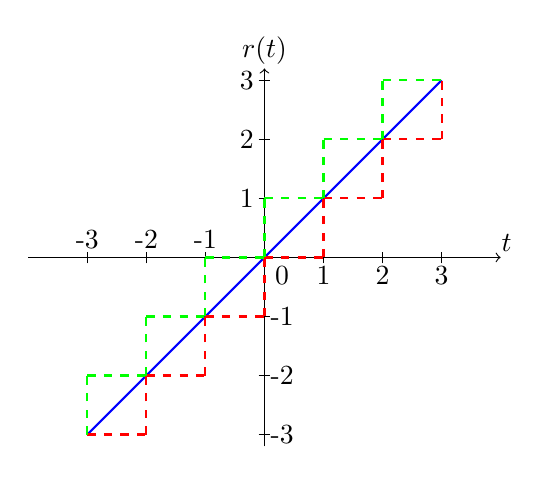
\begin{tikzpicture}
\begin{scope}[scale = 0.75]
\draw[->] (-4,0)-- (4,0);
\draw (0.3,-0.3) node {0};
\draw[->] (0,-3.2)-- (0,3.2);
\draw (4.1,0.25) node {$t$};
\draw (0,3.5) node {$r(t)$};

\draw (1,-0.1)-- (1,0.1);
\draw (1.0,-0.3) node {1};
\draw (2,-0.1)-- (2,0.1);
\draw (2.0,-0.3) node {2};
\draw (3,-0.1)-- (3,0.1);
\draw (3.0,-0.3) node {3};

\draw (-1,-0.1)-- (-1,0.1);
\draw (-1.0,0.3) node {-1};
\draw (-2,-0.1)-- (-2,0.1);
\draw (-2.0,0.3) node {-2};
\draw (-3,-0.1)-- (-3,0.1);
\draw (-3.0,0.3) node {-3};

\draw (-0.1,1)-- (0.1,1);
\draw (-0.3,1) node {1};
\draw (-0.1,2)-- (0.1,2);
\draw (-0.3,2) node {2};
\draw (-0.1,3)-- (0.1,3);
\draw (-0.3,3) node {3};

\draw (-0.1,-1)-- (0.1,-1);
\draw (0.3,-1) node {-1};
\draw (-0.1,-2)-- (0.1,-2);
\draw (0.3,-2) node {-2};
\draw (-0.1,-3)-- (0.1,-3);
\draw (0.3,-3) node {-3};

%r(t)
\draw[thick,blue] (-3,-3)-- (3,3);

\draw[thick,dashed,red] (-3,-3)-- (-2,-3);
\draw[thick,dashed,red] (-2,-3)-- (-2,-2);
\draw[thick,dashed,red] (-2,-2)-- (-1,-2);
\draw[thick,dashed,red] (-1,-2)-- (-1,-1);
\draw[thick,dashed,red] (-1,-1)-- (-0,-1);
\draw[thick,dashed,red] (-0,-1)-- (-0,-0);
\draw[thick,dashed,red] (-0,-0)-- (1,-0);
\draw[thick,dashed,red] (1,0)-- (1,1);
\draw[thick,dashed,red] (1,1)-- (2,1);
\draw[thick,dashed,red] (2,1)-- (2,2);
\draw[thick,dashed,red] (2,2)-- (3,2);
\draw[thick,dashed,red] (3,2)-- (3,3);

\draw[thick,dashed,green] (-3,-2)-- (-2,-2);
\draw[thick,dashed,green] (-3,-3)-- (-3,-2);
\draw[thick,dashed,green] (-2,-1)-- (-1,-1);
\draw[thick,dashed,green] (-2,-2)-- (-2,-1);
\draw[thick,dashed,green] (-1,-0)-- (-0,-0);
\draw[thick,dashed,green] (-1,-1)-- (-1,0);
\draw[thick,dashed,green] (-0,1)-- (1,1);
\draw[thick,dashed,green] (0,0)-- (0,1);
\draw[thick,dashed,green] (1,2)-- (2,2);
\draw[thick,dashed,green] (1,1)-- (1,2);
\draw[thick,dashed,green] (2,3)-- (3,3);
\draw[thick,dashed,green] (2,2)-- (2,3);
\end{scope}
\end{tikzpicture}
\end{center}
}
\vspace{0.3cm}
\only<3->{
Ici le quanta vaut 1 unité et la gamme dynamique est de 6 quanta
}

\end{frame}

\begin{frame}
\frametitle{Codage} 
\textbf{Exercice: Supposons qu'on code un signal d'une amplitude de crête de 5 volts sur 4 bits}\\
\vspace{1cm}
\begin{itemize}
\item<2-> De combien de valeurs dispose-t-on pour coder la gamme dynamique ?  \only<4->{\textbf{16 valeurs: [0,15]}}
\item<3-> Quelle est la valeur d'un quanta/échelon de quantification ? \only<5->{$q$ = \textbf{0.625 V}} 
\end{itemize}

\end{frame} 

\subsubsection{Echantillonnage} 
\begin{frame} 
\frametitle{\'Echantillonnage} 

\textbf{Question : En quoi consiste pour vous l'opération d'échantillonnage ?}

\only<2->{
\begin{block}{}
"L’échantillonnage consiste à représenter un signal fonction du temps $s(t)$ par ses
valeurs $s(nT_e)$ à des instants multiples entiers d’une durée $T_e$, appelée période d’échantillonnage."\footnotesize {M. Bellanger}
\end{block}
}
\end{frame}

\begin{frame}
\frametitle{\'Echantillonnage : Peigne de Dirac}

L'opération d'échantillonnage s'appuie sur la distribution appelée "peigne de Dirac"\\

\vspace{0.7cm} 

 \[ u_{T_e}(t) = \sum_{n = -\infty}^{\infty} \delta(t-nT_e) \]\\
 
\vspace{0.7cm}
On a alors\\

\vspace{0.3cm}
\begin{block}{}
 \[s(nT_e) = s(t) \cdot u_{T_e}(t) \]
\end{block}

\end{frame} 

\begin{frame}
\frametitle{\'Echantillonnage: exemple}
On souhaite échantillonner le signal : $$ g(t) = 0.55\cos(2 t) + 0.45 \cos(4 t + \frac{\pi}{3}) $$ 
\only<2->{
\begin{center}
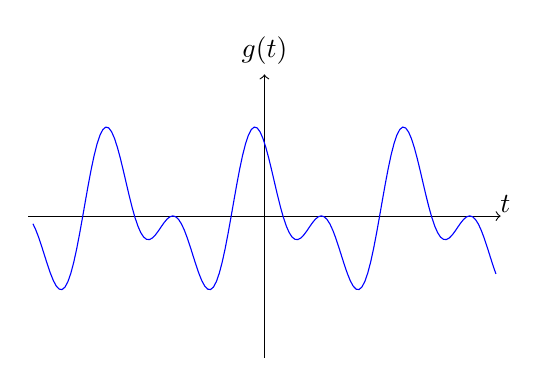
\begin{tikzpicture}
\begin{scope}[scale=0.6]
	\draw[->] (-5,0)-- (5,0);
%\draw (-0.3,-0.3) node {0};
\draw[->] (0,-3)-- (0,3);
\draw (5.1,0.25) node {$t$};
\draw (0,3.5) node {$g(t)$};
%\draw (4.5,-0.3) node {1};

\draw[domain=-4.9:4.9,color=blue,samples=160] plot (\x,{2*(0.55*cos(2*\x r)+ 0.45*cos(2*2*(\x+3.14/12) r))});
\end{scope}
	\end{tikzpicture}
\end{center}
}

\only<3->
{
\begin{block}{}
Quelles sont les composantes en fréquences de ce signal ?
\end{block}
}
\end{frame}

\begin{frame}
\frametitle{\'Echantillonnage: exemple}
On souhaite échantillonner le signal : $$ g(t) = 0.55\cos(2 t) + 0.45 \cos(4 t + \frac{\pi}{3}) $$ 
\only<2->{
\begin{center}
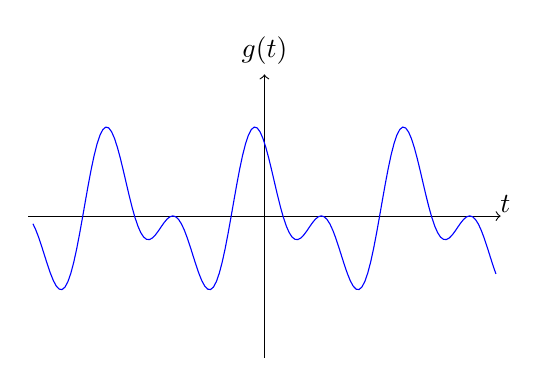
\begin{tikzpicture}
\begin{scope}[scale=0.6]
	\draw[->] (-5,0)-- (5,0);
%\draw (-0.3,-0.3) node {0};
\draw[->] (0,-3)-- (0,3);
\draw (5.1,0.25) node {$t$};
\draw (0,3.5) node {$g(t)$};
%\draw (4.5,-0.3) node {1};

\draw[domain=-4.9:4.9,color=blue,samples=160] plot (\x,{2*(0.55*cos(2*\x r)+ 0.45*cos(2*2*(\x+3.14/12) r))});
\end{scope}
	\end{tikzpicture}
\end{center}
}

\only<3->
{
\begin{block}{}
Quelles sont les composantes en fréquences de ce signal ?
\end{block}
}
\end{frame}

\begin{frame}
\frametitle{\'Echantillonnage: exemple}
On souhaite échantillonner le signal : $$g(t) = 0.55\cos(2 t) + 0.45 \cos(4 t + \frac{\pi}{3}) $$
\begin{columns}[T]
\column{60 mm}
\begin{center}
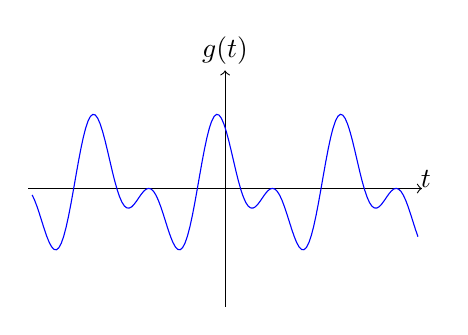
\begin{tikzpicture}
\begin{scope}[scale=0.5,yshift=-1cm]
	\draw[->] (-5,0)-- (5,0);
%\draw (-0.3,-0.3) node {0};
\draw[->] (0,-3)-- (0,3);
\draw (5.1,0.25) node {$t$};
\draw (0,3.5) node {$g(t)$};
%\draw (4.5,-0.3) node {1};

\draw[domain=-4.9:4.9,color=blue,samples=160] plot (\x,{2*(0.55*cos(2*\x r)+ 0.45*cos(2*2*(\x+3.14/12) r))});
\end{scope}
	\end{tikzpicture}
\end{center}

\column{60 mm}

Quelles sont les composantes en fréquence de ce signal ?
\begin{itemize}
\item Méthode "directe" 
\item<2-> Transformée de Fourier 
\end{itemize}
\vspace{0.3cm}
\only<3->
{
$f_1 = \frac{\displaystyle 1}{\displaystyle \pi}$,   $f_2 = \frac{\displaystyle 2}{\displaystyle \pi}$\\
}

\end{columns}
\end{frame}


\begin{frame}
\frametitle{\'Echantillonnage: exemple}
On souhaite échantillonner le signal : $$g(t) = 0.55\cos(2 t) + 0.45 \cos(4 t + \frac{\pi}{3}) $$
\begin{columns}[T]
\column{60 mm}
\begin{center}
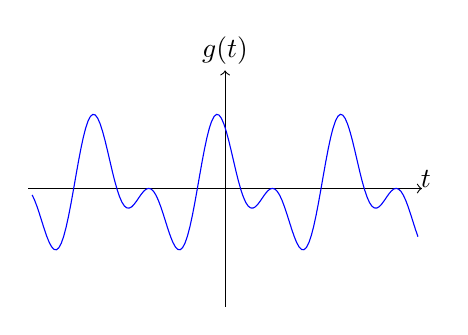
\begin{tikzpicture}
\begin{scope}[scale=0.5,yshift=-1cm]
	\draw[->] (-5,0)-- (5,0);
%\draw (-0.3,-0.3) node {0};
\draw[->] (0,-3)-- (0,3);
\draw (5.1,0.25) node {$t$};
\draw (0,3.5) node {$g(t)$};
%\draw (4.5,-0.3) node {1};

\draw[domain=-4.9:4.9,color=blue,samples=160] plot (\x,{2*(0.55*cos(2*\x r)+ 0.45*cos(2*2*(\x+3.14/12) r))});
\end{scope}
	\end{tikzpicture}
\end{center}

\column{60 mm}

$f_1 = \frac{\displaystyle 1}{\displaystyle \pi}$,   $f_2 = \frac{\displaystyle 2}{\displaystyle \pi}$\\

\vspace{0.3cm}

\only<2->{
Que faut-il avoir à l'esprit lors du choix de $f_e$ (fréquence d'échantillonnage) ?
}

\end{columns}
\end{frame}

\begin{frame} 
\frametitle{\'Echantillonnage: exemple}
\begin{block}{Critère de Shannon}
Pour échantillonner un signal sans perte d'information, il faut que la fréquence d'échantillonnage soit deux fois supérieure à la fréquence maximale présente dans le signal
\end{block}
\only<2->{
\vspace{0.3cm}
$g(t) = 0.55\cos(2 t) + 0.45 \cos(4 t + \frac{\pi}{3}) \rightarrow f_e = $ ?
}

\only<3->{
\vspace{0.3cm}
$g(t) = 0.55\cos(2 t) + 0.45 \cos(4 t + \frac{\pi}{3}) \rightarrow f_e \geq 4/\pi $ 
}

\end{frame}

\begin{frame}
\frametitle{\'Echantillonnage: exemple}
\begin{columns}
\column{60mm}
\begin{center}
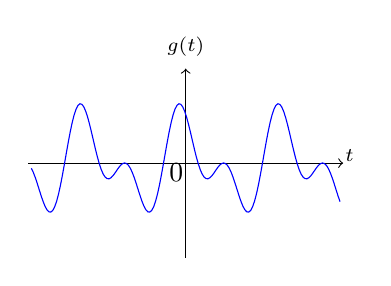
\begin{tikzpicture}
\begin{scope}[scale=0.4]
	\draw[->] (-5,0)-- (5,0);
\draw (-0.3,-0.3) node {0};
\draw[->] (0,-3)-- (0,3);
\draw (5.2,0.25) node {\scriptsize $t$};
\draw (0,3.7) node {\scriptsize $g(t)$};
%\draw (4.5,-0.3) node {1};

\draw[domain=-4.9:4.9,color=blue,samples=160] plot (\x,{2*(0.55*cos(2*\x r)+ 0.45*cos(2*2*(\x+3.14/12) r))});
\end{scope}
	\end{tikzpicture}
\end{center}
\column{60mm}
\begin{center}
\begin{tikzpicture}
\begin{scope}[scale=0.4]
	\draw[->] (-5,0)-- (5,0);
%\draw (-0.3,-0.3) node {0};
\draw[->] (0,-3)-- (0,3);
\draw (5.3,0.25) node {\scriptsize $t$};
\draw (0,3.7) node {\scriptsize $u_{T_e}(t)$};
%\draw (4.5,-0.3) node {1};

\draw[thick,blue] (-4,-0)-- (-4,1);
\draw[thick,blue] (-3.5,-0)-- (-3.5,1);
\draw[thick,blue] (-3,-0)-- (-3,1);
\draw[thick,blue] (-2.5,-0)-- (-2.5,1);
\draw[thick,blue] (-2,-0)-- (-2,1);
\draw[thick,blue] (-1.5,-0)-- (-1.5,1);
\draw[thick,blue] (-1,-0)-- (-1,1);
\draw[thick,blue] (-0.5,-0)-- (-0.5,1);
\draw[thick,blue] (0,-0)-- (0,1);
\draw[thick,blue] (0.5,-0)-- (0.5,1);
\draw[thick,blue] (1,-0)-- (1,1);
\draw[thick,blue] (1.5,-0)-- (1.5,1);
\draw[thick,blue] (2,-0)-- (2,1);
\draw[thick,blue] (2.5,-0)-- (2.5,1);
\draw[thick,blue] (3,-0)-- (3,1);
\draw[thick,blue] (3.5,-0)-- (3.5,1);
\draw[thick,blue] (4,-0)-- (4,1);
\end{scope}
	\end{tikzpicture}
\end{center}

\end{columns}

\begin{center}
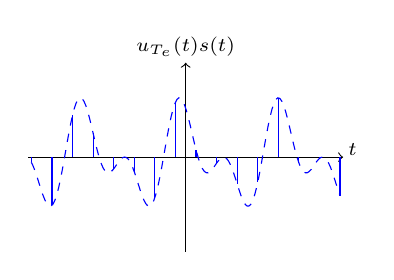
\begin{tikzpicture}
\begin{scope}[scale=0.4]
	\draw[->] (-5,0)-- (5,0);
%\draw (-0.3,-0.3) node {0};
\draw[->] (0,-3)-- (0,3);
\draw (5.3,0.25) node {\scriptsize $t$};
\draw (0,3.5) node {\scriptsize $u_{T_{e}}(t)s(t)$};
%\draw (4.5,-0.3) node {1};

\draw[dashed,domain=-4.9:4.9,color=blue,samples=160] plot (\x,{2*(0.55*cos(2*\x r)+ 0.45*cos(2*2*(\x+3.14/12) r))});

\draw[domain=-4.9:4.9,color=blue,samples=16] plot[ycomb] (\x,{2*(0.55*cos(2*\x r)+ 0.45*cos(2*2*(\x+3.14/12) r))});
%\draw[ domain=0.1:4.9,color=blue,samples=24] plot[ycomb] (\x,{80*abs(sin(5*3.14*\x r -5*3.14*2.5r )/(5*3.14*\x r-5*3.14*2.5 r))});
%\draw[thick,blue] (-4,-0)-- (-4,-0.9);
%\draw[thick,blue] (-3,-0)-- (-3,1);
%\draw[thick,blue] (-2,-0)-- (-2,0);
%\draw[thick,blue] (-1,-0)-- (-1,-1.25);
%\draw[thick,blue] (0,-0)-- (0,1.3);
%\draw[thick,blue] (1,-0)-- (1,-0.15);
%\draw[thick,blue] (2,-0)-- (2,-1.5);
%\draw[thick,blue] (3,-0)-- (3,1.8);
%\draw[thick,blue] (4,-0)-- (4,-0.35);
\end{scope}
	\end{tikzpicture}
\end{center}
\end{frame}

\begin{frame}
\frametitle{\'Echantillonnage: exemple}
Dans les faits, respecter Shannon strictement est un peu limite...\\

\vspace{0.5cm}
\begin{columns}
\column{60mm}
\begin{center}
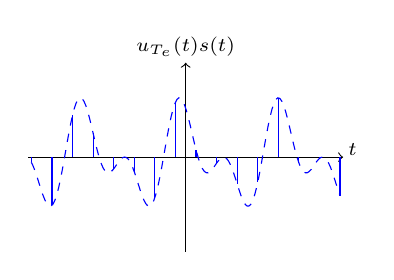
\begin{tikzpicture}
\begin{scope}[scale=0.4]
	\draw[->] (-5,0)-- (5,0);
%\draw (-0.3,-0.3) node {0};
\draw[->] (0,-3)-- (0,3);
\draw (5.3,0.25) node {\scriptsize $t$};
\draw (0,3.5) node {\scriptsize $u_{T_{e}}(t)s(t)$};
%\draw (4.5,-0.3) node {1};

\draw[dashed,domain=-4.9:4.9,color=blue,samples=160] plot (\x,{2*(0.55*cos(2*\x r)+ 0.45*cos(2*2*(\x+3.14/12) r))});

\draw[domain=-4.9:4.9,color=blue,samples=16] plot[ycomb] (\x,{2*(0.55*cos(2*\x r)+ 0.45*cos(2*2*(\x+3.14/12) r))});
%\draw[ domain=0.1:4.9,color=blue,samples=24] plot[ycomb] (\x,{80*abs(sin(5*3.14*\x r -5*3.14*2.5r )/(5*3.14*\x r-5*3.14*2.5 r))});
%\draw[thick,blue] (-4,-0)-- (-4,-0.9);
%\draw[thick,blue] (-3,-0)-- (-3,1);
%\draw[thick,blue] (-2,-0)-- (-2,0);
%\draw[thick,blue] (-1,-0)-- (-1,-1.25);
%\draw[thick,blue] (0,-0)-- (0,1.3);
%\draw[thick,blue] (1,-0)-- (1,-0.15);
%\draw[thick,blue] (2,-0)-- (2,-1.5);
%\draw[thick,blue] (3,-0)-- (3,1.8);
%\draw[thick,blue] (4,-0)-- (4,-0.35);
\end{scope}
\end{tikzpicture}
\end{center}

\column{60mm}
\begin{center}
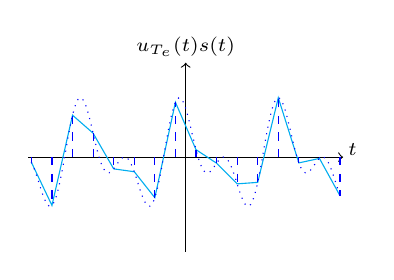
\begin{tikzpicture}
\begin{scope}[scale=0.4]
	\draw[->] (-5,0)-- (5,0);
%\draw (-0.3,-0.3) node {0};
\draw[->] (0,-3)-- (0,3);
\draw (5.3,0.25) node {\scriptsize $t$};
\draw (0,3.5) node {\scriptsize $u_{T_{e}}(t)s(t)$};
%\draw (4.5,-0.3) node {1};

\draw[domain=-4.9:4.9,color=cyan,samples=16] plot (\x,{2*(0.55*cos(2*\x r)+ 0.45*cos(2*2*(\x+3.14/12) r))});

\draw[dotted,domain=-4.9:4.9,color=blue,samples=160] plot (\x,{2*(0.55*cos(2*\x r)+ 0.45*cos(2*2*(\x+3.14/12) r))});

\draw[dashed,domain=-4.9:4.9,color=blue,samples=16] plot[ycomb] (\x,{2*(0.55*cos(2*\x r)+ 0.45*cos(2*2*(\x+3.14/12) r))});
%\draw[ domain=0.1:4.9,color=blue,samples=24] plot[ycomb] (\x,{80*abs(sin(5*3.14*\x r -5*3.14*2.5r )/(5*3.14*\x r-5*3.14*2.5 r))});
%\draw[thick,blue] (-4,-0)-- (-4,-0.9);
%\draw[thick,blue] (-3,-0)-- (-3,1);
%\draw[thick,blue] (-2,-0)-- (-2,0);
%\draw[thick,blue] (-1,-0)-- (-1,-1.25);
%\draw[thick,blue] (0,-0)-- (0,1.3);
%\draw[thick,blue] (1,-0)-- (1,-0.15);
%\draw[thick,blue] (2,-0)-- (2,-1.5);
%\draw[thick,blue] (3,-0)-- (3,1.8);
%\draw[thick,blue] (4,-0)-- (4,-0.35);
\end{scope}
\end{tikzpicture}
\end{center}

\end{columns}

\begin{block}{}
Dans les faits on prend plutôt $f_e > 5 f_{max}$ voire $f_e > 10 f_ {max}$
\end{block}

\end{frame}

\begin{frame}
\frametitle{Impact de l'échantillonnage sur le spectre}

Soit une fonction $g(t)$, $g_{T_e}(nT_e) = \sum_{n = -\infty}^{\infty} g(t)\delta(t-nT_e))$, alors \\

\vspace{1cm} 

\[ TF (\sum_{n = -\infty}^{\infty} g(t)\delta(t-nT_e)) = \frac{1}{T}\sum_{n = -\infty}^{\infty} G(f) \star \delta(f - \frac{n}{T_e}) \] 

\vspace{0.5cm}

\begin{block}{}
Le spectre du signal échantillonnée est constitué de répétitions du spectre du signal original répété tous les $f_e = \frac{1}{T_e}$
\end{block}


\end{frame}

\begin{frame}
\frametitle{Impact de l'échantillonnage sur le spectre}
\vspace{0.5cm}
\begin{columns}
\column{60mm}
\begin{center}
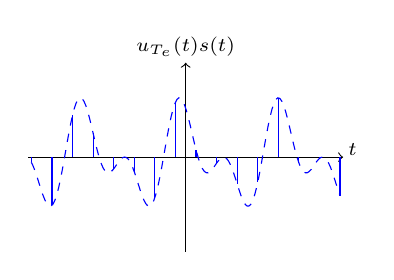
\begin{tikzpicture}
\begin{scope}[scale=0.4]
	\draw[->] (-5,0)-- (5,0);
%\draw (-0.3,-0.3) node {0};
\draw[->] (0,-3)-- (0,3);
\draw (5.3,0.25) node {\scriptsize $t$};
\draw (0,3.5) node {\scriptsize $u_{T_{e}}(t)s(t)$};
%\draw (4.5,-0.3) node {1};

\draw[dashed,domain=-4.9:4.9,color=blue,samples=160] plot (\x,{2*(0.55*cos(2*\x r)+ 0.45*cos(2*2*(\x+3.14/12) r))});

\draw[domain=-4.9:4.9,color=blue,samples=16] plot[ycomb] (\x,{2*(0.55*cos(2*\x r)+ 0.45*cos(2*2*(\x+3.14/12) r))});

\end{scope}
\end{tikzpicture}

\only<2->{
\begin{center}
\begin{tikzpicture}
\begin{scope}[scale=0.4]
	\draw[->] (-5,0)-- (5,0);
\draw (-0,-0.3) node {\scriptsize 0};
\draw[->] (0,0)-- (0,3);
\draw (5.2,0.25) node {\scriptsize $f$};
\draw (0,3.5) node {\scriptsize $|G(f)|$};
%\draw (4.5,-0.3) node {1};


\draw[thick,blue] (1.05,0)-- (1.05,2.5*0.55);
\draw[thick,blue] (2.05,0)-- (2.05,2.5*0.45);
\draw (2.1,-0.8) node {\scriptsize $\frac{2}{\pi}$};
\draw (1.1,-0.8) node {\scriptsize $\frac{1}{\pi}$};

\draw[thick,blue] (-1.05,0)-- (-1.05,2.5*0.55);
\draw[thick,blue] (-2.05,0)-- (-2.05,2.5*0.45);
\draw (-2.1,-0.8) node { \scriptsize $-\frac{2}{\pi}$};
\draw (-1.1,-0.8) node {\scriptsize $-\frac{1}{\pi}$};
\end{scope}
	\end{tikzpicture}
\end{center}

}
\end{center}

\column{60mm}
\begin{center}
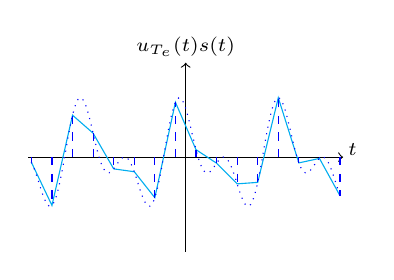
\begin{tikzpicture}
\begin{scope}[scale=0.4]
	\draw[->] (-5,0)-- (5,0);
%\draw (-0.3,-0.3) node {0};
\draw[->] (0,-3)-- (0,3);
\draw (5.3,0.25) node {\scriptsize $t$};
\draw (0,3.5) node {\scriptsize $u_{T_{e}}(t)s(t)$};
%\draw (4.5,-0.3) node {1};

\draw[domain=-4.9:4.9,color=cyan,samples=16] plot (\x,{2*(0.55*cos(2*\x r)+ 0.45*cos(2*2*(\x+3.14/12) r))});

\draw[dotted,domain=-4.9:4.9,color=blue,samples=160] plot (\x,{2*(0.55*cos(2*\x r)+ 0.45*cos(2*2*(\x+3.14/12) r))});

\draw[dashed,domain=-4.9:4.9,color=blue,samples=16] plot[ycomb] (\x,{2*(0.55*cos(2*\x r)+ 0.45*cos(2*2*(\x+3.14/12) r))});

\end{scope}
\end{tikzpicture}

\only<2->{
\begin{center}
\begin{tikzpicture}
\begin{scope}[scale=0.4]
	\draw[->] (-7,0)-- (7,0);
\draw (-0,-0.3) node {\scriptsize 0};
\draw[->] (0,0)-- (0,3);
\draw (7.2,0.25) node {\scriptsize $f$};
\draw (0,3.5) node {\scriptsize $|G(f)|$};
%\draw (4.5,-0.3) node {1};


\draw[thick,blue] (1.05,0)-- (1.05,2.5*0.55);
\draw[thick,blue] (2.05,0)-- (2.05,2.5*0.45);
\draw (2.1,-0.6) node {\scriptsize $\frac{2}{\pi}$};
%\draw (1.1,-0.4) node {$\frac{1}{\pi}$};

\draw[thick,blue] (-1.05,0)-- (-1.05,2.5*0.55);
\draw[thick,blue] (-2.05,0)-- (-2.05,2.5*0.45);
%\draw (-2.1,-0.4) node {$-\frac{2}{\pi}$};
%\draw (-1.1,-0.4) node {$-\frac{1}{\pi}$};


%replica 1
\draw[thick,cyan] (5.05,0)-- (5.05,2.5*0.55);
\draw[thick,cyan] (6.05,0)-- (6.05,2.5*0.45);
%\draw (5.1,-0.4) node {$\frac{5}{\pi}$};
%\draw (6.1,-0.4) node {$\frac{6}{\pi}$};

\draw[thick,cyan] (3.05,0)-- (3.05,2.5*0.55);
\draw[thick,cyan] (2.08,0)-- (2.08,2.5*0.45);
%\draw (3.1,-0.4) node {$\frac{3}{\pi}$};
%\draw (2.1,-0.4) node {$\frac{1}{\pi}$};
\draw (4.1,-0.8) node { \scriptsize $\frac{4}{\pi}$};


%replica 2
\draw[thick,cyan] (-5.05,0)-- (-5.05,2.5*0.55);
\draw[thick,cyan] (-6.05,0)-- (-6.05,2.5*0.45);
%\draw (-5.1,-0.4) node {$-\frac{5}{\pi}$};
%\draw (-6.1,-0.4) node {$-\frac{6}{\pi}$};

\draw[thick,cyan] (-3.05,0)-- (-3.05,2.5*0.55);
\draw[thick,cyan] (-2.08,0)-- (-2.08,2.5*0.45);
%\draw (-3.1,-0.4) node {$-\frac{3}{\pi}$};
%\draw (2.1,-0.4) node {$\frac{1}{\pi}$};
\draw (-4.1,-0.8) node {\scriptsize $-\frac{4}{\pi}$};
\end{scope}
	\end{tikzpicture}
\end{center}
}
\end{center}

\end{columns}

\only<3->{
\begin{block}{}
On voit que les répliques du spectre se touchent. On est à limite du \textbf{repliement de spectre}
\end{block}
}

\end{frame}

\end{document}
